\begin{table*}
    \begin{tabular}{llp{4cm}}
        \vspace{0.2cm}
        {\bfseries Seite} & {\bfseries Detailauschnitt} & {\bfseries Quelle } \\
        \vspace{0.5cm}
        
        \raisebox{-.5\height}{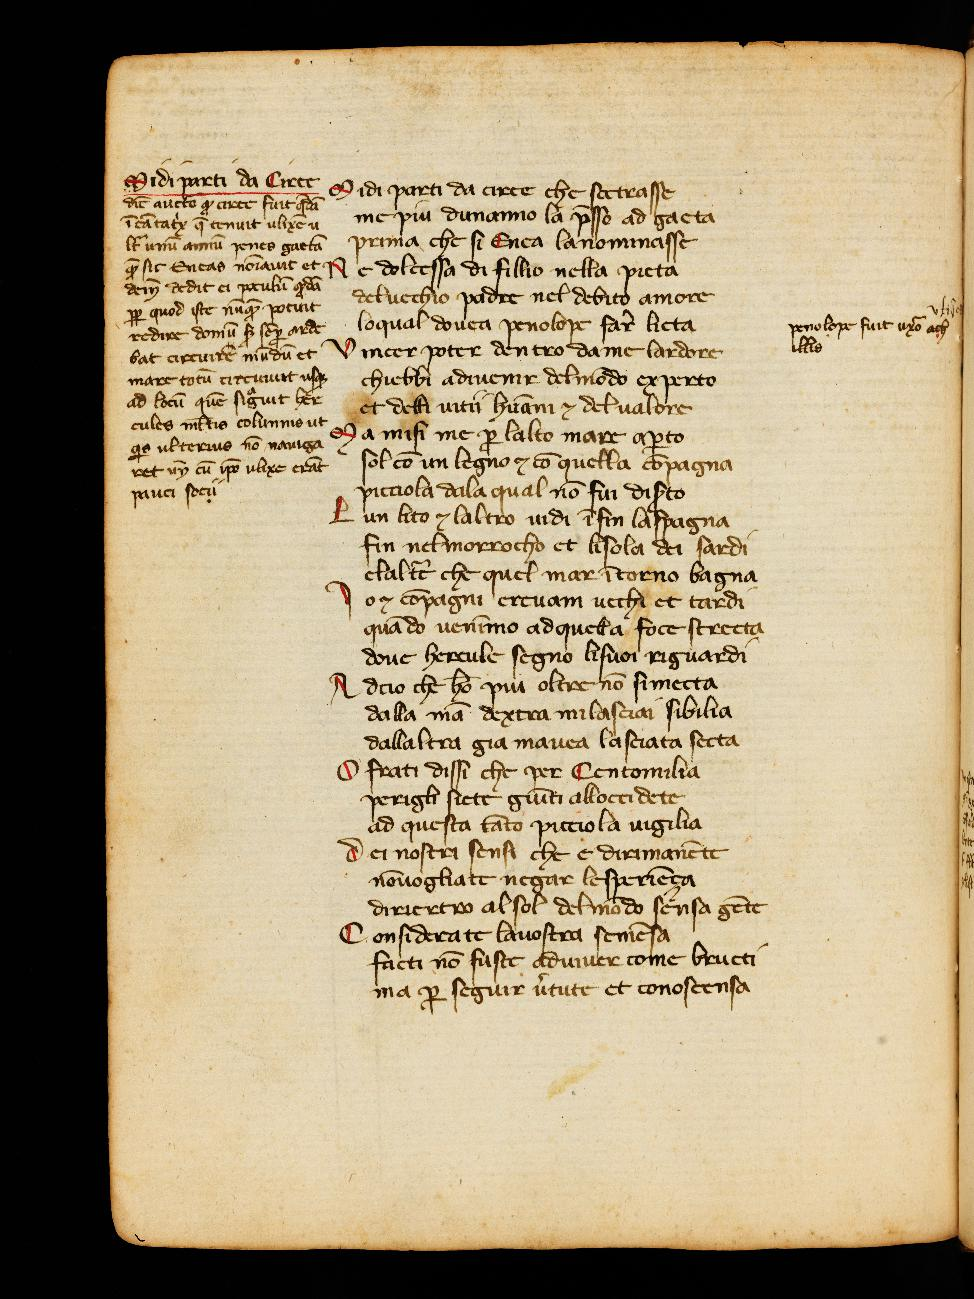
\includegraphics[height=4cm]{figures/datasets/HisDBSample0.jpeg}}
    &\raisebox{-.5\height}{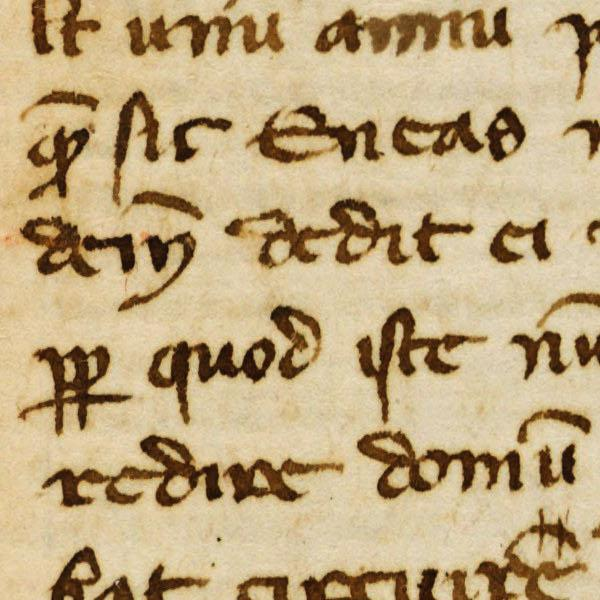
\includegraphics[height=4cm]{figures/datasets/HisDBSampleBox0.jpeg}}
     & \citefield{AlighieriColognyFondationMartin1300}{title}\\
     \vspace{0.5cm}  
     
    \raisebox{-.5\height}{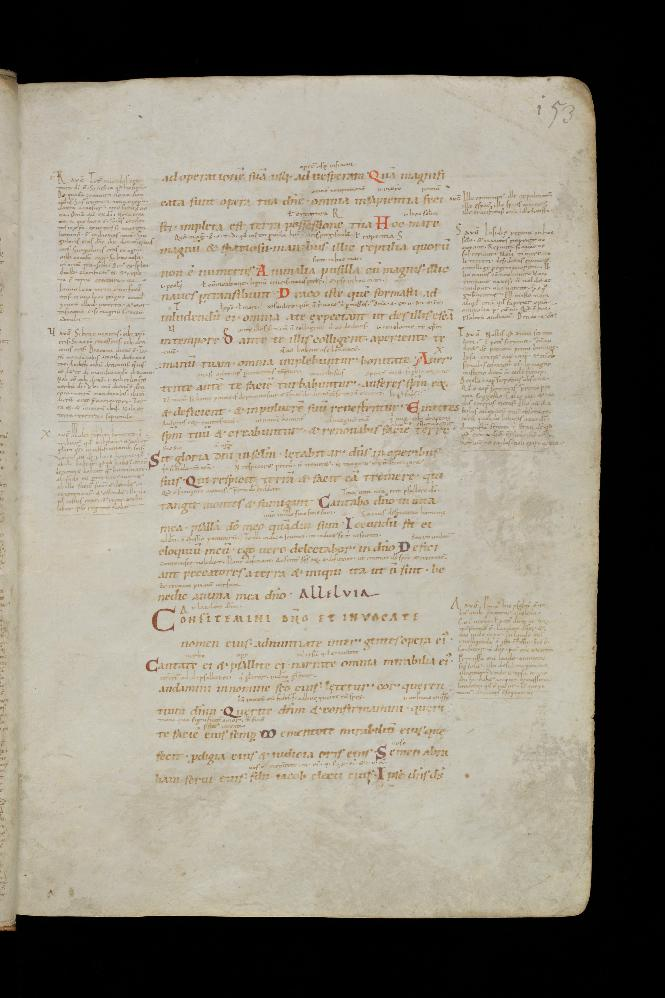
\includegraphics[height=4cm]{figures/datasets/HisDBSample2.jpeg}}
    & \raisebox{-.5\height}{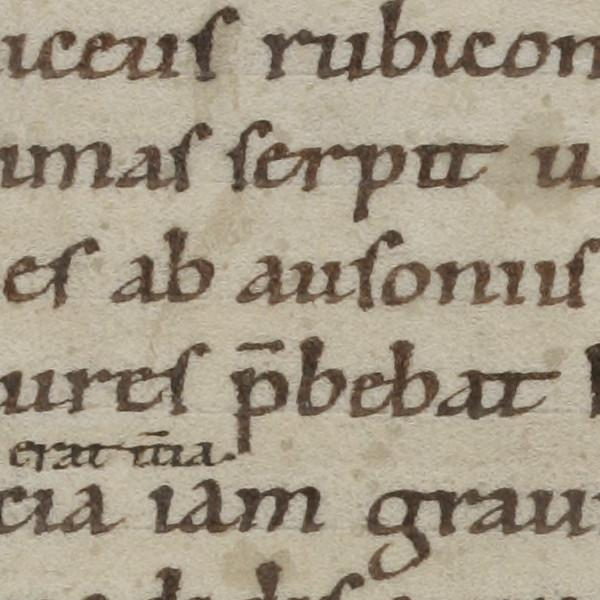
\includegraphics[height=4cm]{figures/datasets/HisDBSampleBox2.jpeg}}
    & \citefield{AmbrosiusStGallenStiftsbibliothek985}{title}\\
    \vspace{0.5cm}
    
     \raisebox{-.5\height}{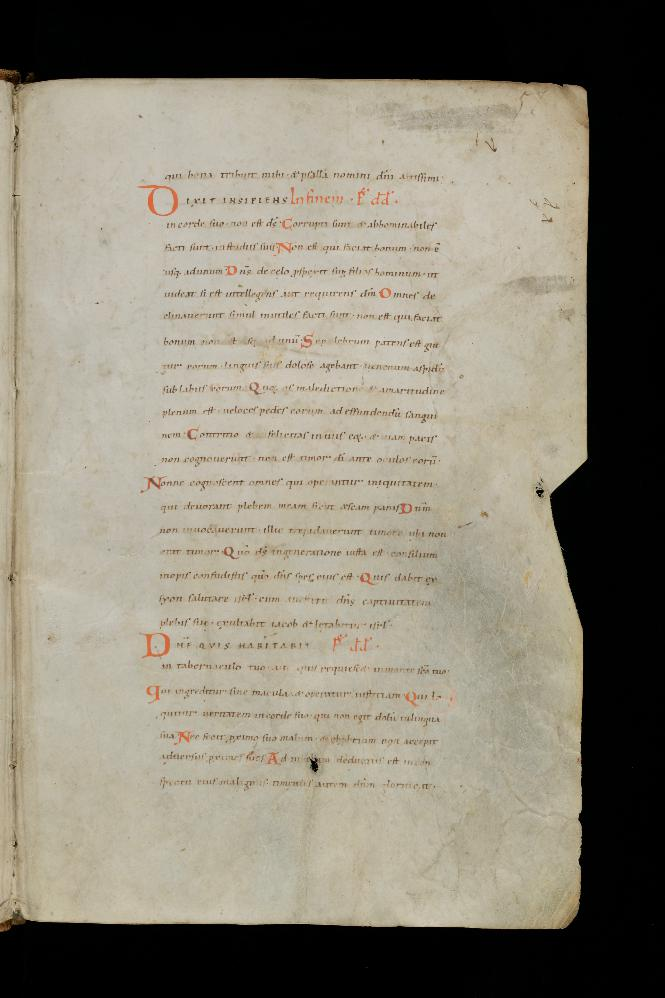
\includegraphics[height=4cm]{figures/datasets/HisDBSample1.jpeg}}
    &\raisebox{-.5\height}{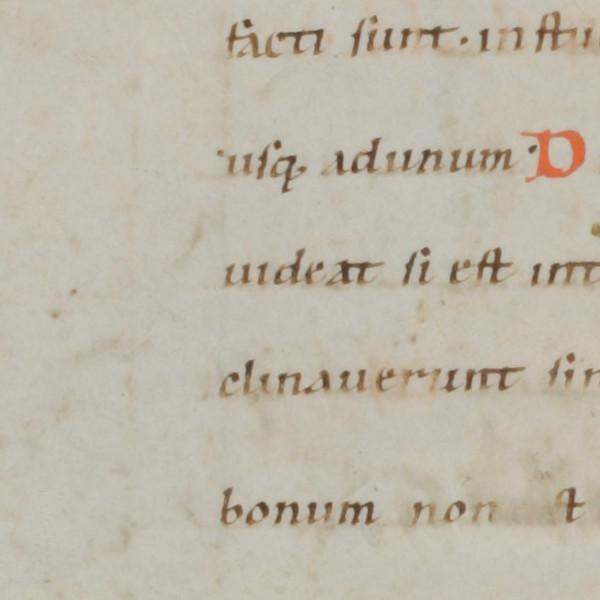
\includegraphics[height=4cm]{figures/datasets/HisDBSampleBox1.jpeg}}
     & \citefield{LucanusStGallenStiftsbibliothek1025}{title}\\
     \vspace{0.5cm} 

    \end{tabular}
    \caption{HisDB Beipsiele mit Detailauschnitt}
    \label{table:hisdbsamples}
\end{table*}